\documentclass[x11names]{article}
\usepackage{tikz}
\usepackage{pgfplots}
\usepackage{xcolor}
\usepackage{svg}
\usepackage{amsmath}
\usepackage{array}
\usepackage[skins]{tcolorbox}
\usepackage[version=4]{mhchem}
\usepackage[a4paper, total={6in, 10in}]{geometry}
\usepackage{fouriernc}
\usepackage{xymtex}
\usepackage{textcomp}
\usepackage{eurosym}
\usepackage{mathrsfs}
\usepackage{float}
\usepackage{pst-all}
\usepackage{pst-3dplot}
\usepackage{leftindex}
\usepackage{verbatim}
\usepackage{import}
\usepackage{xifthen}
\usepackage{pdfpages}
\usepackage{transparent}
\usepackage{import}
\usepackage{pdfpages}
\usepackage{transparent}
\usepackage{amssymb}




% myframe
\newtcolorbox{es}[2][]{%
  enhanced,colback=white,colframe=black,coltitle=black,
  sharp corners,boxrule=0.4pt,
  fonttitle=\itshape,
  attach boxed title to top left={yshift=-0.5\baselineskip-0.4pt,xshift=2mm},
  boxed title style={tile,size=minimal,left=0.5mm,right=0.5mm,
    colback=white,before upper=\strut},
  title=#2,#1
}

\newtcolorbox{blues}[2][]{%
  enhanced,colback=Azure2,colframe=black,coltitle=black,
  sharp corners,boxrule=0.4pt,
  fonttitle=\itshape,
  attach boxed title to top left={yshift=-0.5\baselineskip-0.4pt,xshift=2mm},
  boxed title style={tile,size=minimal,left=0.5mm,right=0.5mm,
    colback=Azure2,before upper=\strut},
  title=#2,#1
}

\newtcolorbox{defin}[2][]{%
  enhanced,colback=white,colframe=LightSkyBlue1,coltitle=black,
  sharp corners,boxrule=1.5pt,
  fonttitle=\itshape,
  attach boxed title to top left={yshift=-0.5\baselineskip-0.4pt,xshift=2mm},
  boxed title style={tile,size=minimal,left=0.5mm,right=0.5mm,
    colback=white,before upper=\strut},
  title=#2,#1
}


%% regole
\renewcommand*\contentsname{Indice}
\setcounter{tocdepth}{4}
\setcounter{secnumdepth}{2}
\pgfplotsset{compat=1.15}


\usetikzlibrary{arrows}


\title{Letteratura italiana}
\author{Federico Cesari}
\date{}



\begin{document}

\begin{titlepage}
	\begin{center}
		\vspace*{1cm}
		
		\textbf{\LARGE Relazione di laboratorio - Pendolo semplice}
		
		\vspace{0.3cm}
		\large \textit{Misura del periodo di un pendolo semplice} \\
		
		\vspace{0.5cm}
		\Large Federico Cesari \\
		
		\small 1096759 
		\vspace{0.2cm}
		
		\small Gruppo 5
		
		
		\vspace{3cm}
		\begin{center}
			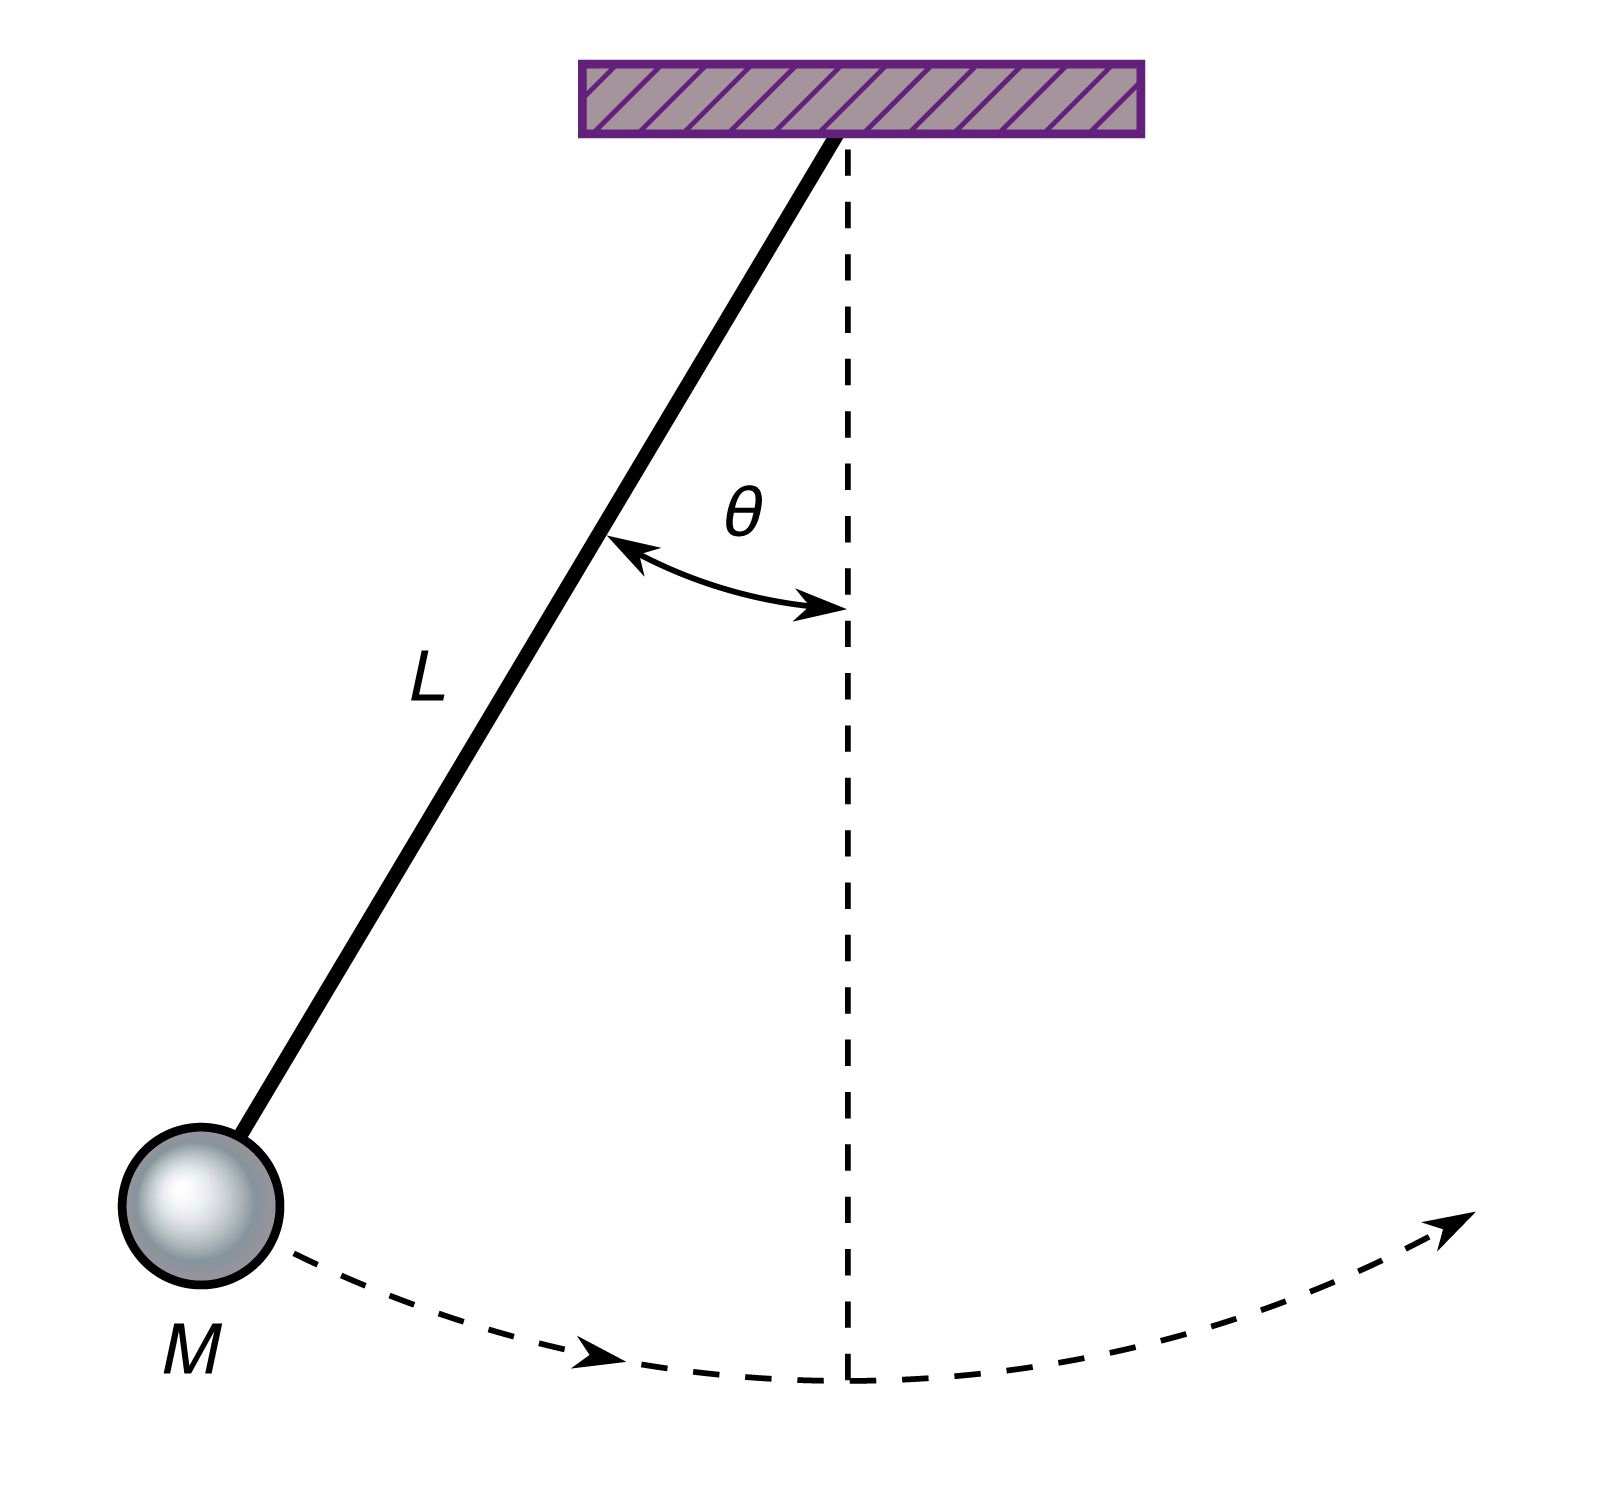
\includegraphics[scale=0.1]{IMG_0200.jpeg}	
		\end{center}
		
		
		
		\vfill
		
		
		
		corso A\\
		Università degli studi di Torino, Torino\\
		4 aprile 2024\\
		
		
	\end{center}
\end{titlepage}
\tableofcontents
\newpage

\section{Numeri Complessi}
L'insieme dei numeri reali può essere esteso con le proprietà delle operazioni di somma e prodotto valide in esso. L'estensione dà vita all'insieme dei numeri complessi che chiamiamo $\mathbb{C}$.

\definecolor{ffqqqq}{rgb}{1,0,0}
\definecolor{ududff}{rgb}{0.30196078431372547,0.30196078431372547,1}
\definecolor{wwqqcc}{rgb}{0.4,0,0.8}
\definecolor{xdxdff}{rgb}{0.49019607843137253,0.49019607843137253,1}
\begin{center}
\begin{tikzpicture}[line cap=round,line join=round,>=triangle 45,x=1cm,y=1cm]
\begin{axis}[
x=1cm,y=1cm,
axis lines=middle,
ymajorgrids=true,
xmajorgrids=true,
xmin=-4,
xmax=4,
ymin=-4,
ymax=4,
ylabel={$i$ }]
\clip(-9.378848871433435,-6.592409255268999) rectangle (14.57608973860068,7.7305174854563585);
\draw [->,line width=1pt,color=xdxdff] (0,0) -- (2,1);
\draw [->,line width=1pt,color=wwqqcc] (0,0) -- (-1,1);
\draw [->,line width=1pt,color=ffqqqq] (0,0) -- (1,2);
\begin{scriptsize}
\draw[color=xdxdff] (1.5040736302530822,0.529963157831875) node {$|z|$};
\draw [fill=xdxdff] (2,1) circle (2.5pt);
\draw[color=xdxdff] (2.692438731011955,1.3586914517821413) node {$z (2,i)$};
\draw [fill=xdxdff] (0,0) circle (2.5pt);
\draw [fill=wwqqcc] (-1,1) circle (2.5pt);
\draw[color=wwqqcc] (-1.4512027387393769,1.5306916637340835) node {$w(-1,i)$};
\draw[color=wwqqcc] (-0.7475655080268867,0.561235923641319) node {$|w|$};
\draw [fill=ududff] (1,2) circle (2.5pt);
\draw [fill=ffqqqq] (1,2) circle (2.5pt);
\draw[color=ffqqqq] (1.066254908920866,2.4845110209221257) node {$z+w$};
\draw[color=ffqqqq] (1.081891291825588,1.3117823030679754) node {$|z+w|$};
\end{scriptsize}
\end{axis}
\end{tikzpicture}       
\end{center}

Questo ampliamento permette la risoluzione di qualsiasi equazione algebrica. Il Teorema Fondamentale dell'algebra afferma che qualsiasi polinomio a coefficienti reali o complessi di grado $n, n \in \mathbb{N}$ ammette almeno una radice complessa, da cui segue che un qualsiasi polinomio a coefficienti reali o complessi di grado $n$ ammette sempre $n$ radici complesse contate con le relative molteplicità.
\\ \\
\noindent
I numeri complessi possono essere indicati con tre differenti notazioni: 
\begin{enumerate}
    \item Cartesiana: $z = (x + iy)$
    \item Trigonometrica: $z = \rho(\cos{\theta} + i\sin{\theta})$
    \item Esponenziale: $z = \rho e^{i\theta}$
\end{enumerate}

\noindent
Ogni notazione ha i suoi vantaggi grafici o di calcolo, per questo preferiremo una notazione ad un'altra in casi specifici. In generale un numero complesso è formato dal una \textit{parte reale $x = Re(z)$} e da una \textit{parte immaginaria $y=Im(z)$}, dal punto di vista algebrico $\mathbb{R} $ e $ \mathbb{C}$ hanno le stesse proprietà anche se nel caso dei numeri complessi non è possibile definire un "ordine" compatibile con le operazioni.

\subsection{Operazioni algebriche}
Le operazioni di somma e differenza sono definite dalla semplice somma o differenza tra parti reali e parti immaginarie. Il prodotto tra due numeri complessi si comporta in modo simile al comportamento di seno e coseno nelle operazioni di somma:
$$
z_1 z_2 = (x_1, y_1)(x_2, y_2) = (x_1 x_2 - y_1 y_2, x_1 y_2 + y_1 x_2)
$$

\vspace{0.7em}
\noindent



Il reciproco di un numero complesso espresso come $\frac{1}{z}$ si può riscrivere moltiplicando sopra e sotto per il complesso coniugato di $z = x - iy$:

\[
\frac{1}{z}\frac{\overline{z}}{\overline{z}} = \frac{x-iy}{x^2 + y^2}
\]

Nel caso di potenze di un numero complesso la notazione esponenziale è particolarmente funzionale. In generale $z^n$ eleva alla $n$ il modulo $\rho$ e l'argomento:

\[
z^n = \rho^n e^{in\theta} =  \rho^n(\cos{n\theta} + i\sin{n\theta}) 
\]

\begin{center}
\fboxsep11pt
\colorbox{Azure2}{\begin{minipage}{5.75in}
Un fatto interessante che spiega perché la parte immaginaria dei numeri complessi è situata a $90^\circ$ in senso antiorario rispetto alla parte reale è che se moltiplichiamo un qualsiasi numero complesso per $i$, questo subirà una rotazione di $90^\circ$ in senso antiorario.
\begin{blues}{es}
Prendiamo $z= 2+i$ e $w=i$:
ora $z \cdot w = (2+i)(i)$  sappiamo essere uguale a $-1 + 2i$.
\begin{center}
\definecolor{qqwwzz}{rgb}{0,0.4,0.6}
\definecolor{wwqqcc}{rgb}{0.4,0,0.8}
\definecolor{xdxdff}{rgb}{0.49019607843137253,0.49019607843137253,1}
\begin{tikzpicture}[line cap=round,line join=round,>=triangle 45,x=1cm,y=1cm]
\begin{axis}[
x=1cm,y=1cm,
axis lines=middle,
ymajorgrids=true,
xmajorgrids=true,
xmin=-5,
xmax=5,
ymin=-5,
ymax=5,
ylabel={$i$}]
\clip(-7.079913199747649,-3.637084505116807) rectangle (8.353685115497054,5.590837202953786);
\draw[line width=0.8pt,color=qqwwzz,fill=qqwwzz,fill opacity=0.1] (0.6371452110745517,0.31857260553727584) -- (0.31857260553727584,0.9557178166118275) -- (-0.31857260553727584,0.6371452110745517) -- (0,0) -- cycle; 
\draw [->,line width=1pt,color=xdxdff] (0,0) -- (2,1);
\draw [->,line width=1pt,color=wwqqcc] (0,0) -- (-1,2);
\draw [shift={(0,0)},line width=0.8pt,color=qqwwzz] (26.56505117707799:0.7123500017505747) arc (26.56505117707799:116.56505117707799:0.7123500017505747);
\draw [shift={(0,0)},line width=0.8pt,color=qqwwzz] (26.56505117707799:0.6619792500689667) arc (26.56505117707799:116.56505117707799:0.6619792500689667);
\begin{scriptsize}
\draw [fill=xdxdff] (2,1) circle (2.5pt);
\draw[color=xdxdff] (2.399862266730984,1.3143603851852632) node {$z (2,i)$};
\draw [fill=wwqqcc] (-1,2) circle (2.5pt);
\draw[color=wwqqcc] (-0.4813447294569957,2.351997869826389) node {$z_1 (-1,2i)$};
\draw[color=qqwwzz] (0.9189621672917079,0.6293181623153938) node {$\theta = 90^\circ$};
\end{scriptsize}
\end{axis}
\end{tikzpicture}    
\end{center}

Sappiamo anche che moltiplicare per $i$ è equivalente a moltiplicare per un certo numero complesso $\cos{\frac{\pi}{2}} + i\sin{\frac{\pi}{2}}$; da ciò notiamo che l'argomento $\theta$ è anche l'angolo di traslazione di un qualsiasi altro numero complesso $l$ moltiplicato per $w$, ovvero per $i$.
\\\\
Quindi possiamo decidere di che angolo traslare qualsiasi numero complesso scegliendo opportunamente l'argomento $\theta$ di un altro numero complesso da moltiplicare.
\end{blues}
\end{minipage}}        
\end{center}

%% LOGICA
\newpage
\section{Logica}
\subsection{Proposizioni}
Definiamo una \textit{proposizione logica} è un enunciato del quale si può inequivocabilmente dire  se  è vero o falso. Attraverso le proposizioni logiche possiamo ottenere operazioni logiche espresse da simboli specifici detti \textit{connettivi logici}: 

\[
\text{negazione logica}\qquad    \neg p \text{("non p")}\\ \\
\]
\[
\text{congiunzione logica}\qquad   p \wedge q  \text{("p e q")}\\ 
\]
\[
\text{disgiunzione logica}\qquad   p \vee q  \text{("p o q")}\\ 
\]

\vspace{0.7em}
\noindent
In matematica molti enunciati sono del tipo "se $p$ è vera, è vera anche $q$" in cui $p$ è condizione sufficiente affinché $q$ sia vera; in questo caso che $q$ sia vera è condizione necessaria affinchè lo sia anche $p$. Questi tipi di enunciati sono detti implicazioni logiche:
\[
\text{implicazione logica}\qquad   p \Rightarrow q  \text{("p implica q")}\\ 
\]
\[
\text{biimplicazione logica}\qquad   p \Longleftrightarrow q  \text{("p equivale a q")}\\ 
\]

\vspace{0.7em}
\noindent
Vengono poi definite delle regole per \textit{negare} le implicazioni o per scriverle in modo logicamente equivalente (nella loro forma \textit{contronominale}):

\[
\text{contronominale}\qquad   (p \Rightarrow q) \Longleftrightarrow (\neg q \Rightarrow \neg p)  
\]

\subsection{Predicati}
Un predicato logico è un enunciato dipendente da uno o più argomenti ed è indicato nella forma $p(x,\dots)$. Gli argomenti $x,\dots$ da cui dipende il predicato rendono quest'ultimo una \textit{proposizione logica} e assume valori di verità Vero o Falso a seconda dei valori assegnati agli argomenti.

\begin{es}{es}
Dato il predicato "$p(x)$ è un numero dispari" con $x \in \mathbb{N}$:

$p(7)$ è Vero, $p(4)$ è Falso.
\end{es}

\vspace{0.7em}
\noindent
Dato un predicato $p(x)$ con $x \in \mathbb{A}$ è naturale chiedersi se l'enunciato $p(x)$ sia vero \textit{per ogni} elemento di A. A questo fine introduciamo dei \textit{quantificatori}:

\[
\forall x, p(x) \qquad \text{("per ogni x, è vero p(x)")}  
\]
\[
\exists x, p(x) \qquad \text{("esiste almeno un x, per cui è vero p(x)")}  
\]
\[
\exists !x, p(x) \qquad \text{("esiste, ed è unico, almeno un x, per cui è vero p(x)")}  
\]

\vspace{0.7em}
\noindent
Anche con in quantificatori sono definite le forme di negazione:

\[
\neg(\forall x, p(x)) \Longleftrightarrow \exists x, \neg p(x)  
\]
\[
\neg(\exists x, p(x)) \Longleftrightarrow \forall x, \neg p(x)
\]

\subsection{Principio di induzione}
Sia $P(n)$ una proprietà che dipende da $n \geq n_0 \geq 0 \quad n,n_0 \in \mathbb{N}$. Ora supponiamo che siano verificate:

\begin{itemize}
    \item $P(n_0)$ è Vero;
    \item $\forall n \geq n_0$, se $P(n)$ è vero, allora $P(n+1)$ è vero.
\end{itemize}

\noindent
Allora  $P(n)$ è vero per ogni $n \geq n_0$.

\begin{es}{es}
Sappiamo che $1+2+3+\dots+n = \frac{n(n+1)}{2}$. Dimostriamo che se e vero per $n$ lo è anche per $n+1$ ($P(n) \Rightarrow P(n+1)$):

\begin{align*}
1+2+3+\dots+n+n+1 & = \frac{(n+1)(n+1+1)}{2} \\ & = \frac{n^2 + n +2n + 2}{2} \\ & = \frac{n^2 + n}{2} + \frac{2n + 2}{2} \\ &=  \frac{n(n+1)}{2} + n+1 
\end{align*}

\end{es}
\vspace{0.7em}
\noindent
Quindi in generale il Principio di induzione si usa in questo modo: prima si controlla che $P(n_0)$ sia vero, poi si assume che sia vero anche per un generico $n$ e, usando tale informazione, si dimostra che anche $P(n+1)$ è vero.

\newpage
\section{Numeri reali}
L'insieme $\mathbb{R}$ è l'ambiente naturale dell'analisi I, nonostante questo non ne conosciamo la definizione rigorosa(!). Possiamo però riflettere sulle sue proprietà:
\begin{itemize}
    \item Si dice che $\mathbb{R}$ sia un \textbf{campo ordinato}. Ovvero sono definite le due \textit{operazioni di somma e prototto} ed è definita una \textit{relazione d'ordine} $x \leq y$ compatibile con le operazioni (cosa non possibile nell'insieme $\mathbb{C}$).
    \item $\mathbb{R}$ è un insieme \textbf{completo}, al suo interno sono inclusi anche i numeri irrazionali.
\end{itemize}

\noindent
\subsection{Completezza di $\mathbb{R}$}

Possiamo dire colloquialmente che $\mathbb{R}$ riempe la retta. Tramite una formulazione più rigorosa notiamo che, dato un certo intervallo, ogni valore successivo è maggiore di un valore nell'intervallo:
\subsubsection{Maggioranti e minoranti}
\noindent
Sia $A \subseteq \mathbb{R}$, si dice che $A$ è:
\begin{itemize}
    \item \textit{superiormente limitato se  $\exists b \in \mathbb{R} | x \leq b, \forall x \in A$}; $\longrightarrow$ esiste un \textbf{maggiorante} di A.
    \item inferiormente limitato se $\exists a \in \mathbb{R} | a \leq x, \forall x \in A$;$\longrightarrow$ esiste un \textbf{minorante} di A.
    \item limitato se $\exists a,b \in \mathbb{R} | a \leq x \leq b, \forall x \in A$;
\end{itemize}

\noindent
Maggiorante e minorante se esistono sicuramente non sono unici: $a,b$ sono infatti ricercati in tutto $\mathbb{R}$; qualunque numero maggiore di un elemento in $A$ è maggiorante e stessa cosa per il minorante.

\subsubsection{Intervalli, massimi e minimi}
\begin{itemize}
    \item Gli intervalli $(-\infty,b) $ e $ (-\infty,b]$ sono limitati superiormente;
    \item Gli intervalli $(b, +\infty) $ e $ [b, +\infty)$ sono limitati inferiormente;
    \item Gli intervalli $(a,b) $ , $ [ab)$ $(a,b) $ , $ [ab]$ sono limitati.
\end{itemize}

\noindent
Sia $A \subseteq \mathbb{R}$ superiormente limitato:
Allora si dice che $A$ ammette un massimo se $\exists x_M \in A | x \leq x_M, \forall x \in A$. La differenza con un maggiorante sta proprio nel fatto che il massimo è contenuto nell'intervallo; la stessa cosa si può dire per i minimi. 
\\\\
\noindent
Esistono casi che però non ammettono massimi o minimi, per esempio l'insieme $\tilde{A} = \{ \frac{1}{n} | n = 1,2,\dots \}$. Quest'ultimo ha come intervallo $[1,+\infty)$, ha quindi un massimo ma non ammette minimi. In questi casi quando $\neg \exists$ minimo o massimo sarebbe utile poter definire un minorante o maggiorante \textit{ottimale} che vengono definiti rispettivamente come \textit{il più grande dei minoranti e il più piccolo dei maggioranti}. Definiamo allora i concetti di \textit{\textbf{estremo superiore}} ed \textit{\textbf{estremo inferiore}}.

\subsection{Intorni}
Un'altra  "struttura" fondamentale di $\mathbb{R}$ è quealla che si basa sul concetto di \textbf{intorno}.
\\\\
\noindent
Dati $x_0\in \mathbb{R} $ e $ r>0$, si dice intorno di centro $x_0$ e raggio $r$ l'intervallo $In(x_0) = (x_0 -r, x_0 +r)$.
\\\\
\noindent
In questo contesto è utile definire anche un \textit{sistema esteso dei numeri reali} che includa anche $+\infty $ e $ +\infty$: $\overline{\mathbb{R}} = \mathbb{R} \cup \{ -\infty,+\infty \}$. 

\newpage
\section{Limiti e continuità}
Nel capitolo precedente abbiamo introdotto il concetto di \textit{intorno}, ora vediamo come questo sia essenziale nella comprensione dei \textbf{limiti}.


\begin{center}
\fboxsep11pt
\colorbox{Azure2}{\begin{minipage}{5.75in}
\begin{blues}{Definizione: Limite}
Si dice che $\lim_{x\to x_0}f\left(x\right) = l$ se e solo se: \\
$\forall$ intorno di $l, I\left(l\right)$ $\exists$ intorno di $x_0, I\left(x_0\right)$ tale che $\quad x \in I\left(x_0\right) \backslash\{x_0\} \quad \Rightarrow \quad f\left(x\right) \in I\left(l\right)$ 
\end{blues}
\end{minipage}}       
\end{center}




Adesso dobbiamo stabilire alcune proprietà del limite: intanto se esiste il limite \textit{è unico}, possiamo dire infatti "il limite di $f$" e non "uno dei limiti di $f$".

\subsubsection{Teorema di unicità del limite} Supponiamo che $f$ ammetta limite $l$ fiinto o infinito per $x$ tendente a $x_0$. ALlora $f$ non ha altri limiti tendenti a $x_0$.

\begin{es}{dimostrazione: unicità del limite} 
Supponiamo che esistano due limiti differenti di una funzione $f$ tendente allo stesso valore $x_0$ e li chiamiamo $l_1$ e $l_2$ tali che $\lim_{x\to x_0}f\left(x\right) = l_1$ e $\lim_{ x\to x_0}f\left(x\right) = l_2$. Inoltre prendiamo gli intorni di  $l_1$ e di $l_2$ in modo che $l_1 \cap l_2 = \varnothing$.
	
\begin{center}
\includesvg[scale=0.3]{figures/intornielle}
\end{center}


Ora dalla definizione di limite data prima, possiamo scrivere:
\begin{enumerate}
	\item $\lim_{x\to x_0}f\left(x\right) = l_1 \quad \Rightarrow \quad  \exists I\left(x_0\right) | x \in I\left(x_0\right) \backslash \{x_0\} \quad \Rightarrow \quad f\left(x\right) \in I\left(l_1\right)$
	\item $\lim_{x\to x_0}f\left(x\right) = l_2 \quad \Rightarrow \quad  \exists I'\left(x_0\right) | x \in I'\left(x_0\right) \backslash \{x_0\} \quad \Rightarrow \quad f\left(x\right) \in I\left(l_2\right)$
\end{enumerate}
\end{es}


\newpage
\section{Proprietà e calcolo dei limiti}


\newpage
\section{Confronto locale di funzioni}


\newpage
\section{Proprietà globali delle funzioni continue}
Nei capitoli precedenti ci siamo occupati, mediante il concetto di limite, delle varie proprietà locali di una funzione, ossia proprietà che valgono in un intorno di un punto della retta reale. Ora è necessario parlare di alcune proprietà globali delle funzioni, valide su tutto l'intervallo.

\begin{center}
\fboxsep11pt
\colorbox{Azure2}{\begin{minipage}{5.75in}
\begin{blues}{Definizione: Zero di una funzione}
Data una funzione reale $f$ chiamiamo \textbf{zero} di $f$ ogni punto $x_0 \in$ dom$f$ in cui la funzione si annulla.
\end{blues}
\end{minipage}}        
\end{center}
\subsubsection{Teorema di esistenza degli zeri}
Sia $f:\left[a,b\right] \rightarrow \mathbb{R}$ una funzione \textit{continua} nell'intervallo chiuso e limitato $\left[a,b\right]$. Se la funzione $f$ assume valori di segno discorde agli estremi dell'intervallo, allora esiste uno zero  di $f$ nell'intervallo aperto $\left(a,b\right)$; in formule:
\[
	f\left(a\right)f\left(b\right) < 0 \quad \Rightarrow \quad \exists c \in \left(a,b\right) : f\left(c\right) = 0
.\] 
Inoltre se $f$ è strettamente monotona in $\left[a,b\right]$, allora lo zero è unico nell'intervallo.
\begin{center}
\includesvg[scale=0.8]{figures/zeri_func}
\end{center}

\begin{es}{dimostrazione: teorema esistenza degli zeri}
Supponiamo $f\left(a\right)$ negativo e $f\left(b\right)$ positivo: $f\left(a\right) < 0 < f\left(b\right)$. 
\\ \\
Definiamo poi il punto medio $c_0$ e rinominiamo $a$ e  $b$ : $a = a_0$, $b = b_0$, $c_0=\frac{a_0+b_0}{2}$.
\\
\noindent
Una volta calcolato il punto medio abbiamo tre possibilità:
\begin{enumerate}
	\item Se $f\left(c_0\right) = 0$ il teorema è dimostrato;
	\item Se $f\left(c_0\right) > 0$ allora dovremo cercare lo zero \textit{a sinistra} del punto medio; in questo caso poniamo quindi $a_0 = a_1$ e $c_0=b_1$;
	\item Se $f\left(c_0\right) < 0$ allora dovremo cercare lo zero \textit{a destra} del punto medio; in questo caso poniamo $c_0= a_1$ e $b_0 = b_1$.
\end{enumerate}

\begin{center}
\includesvg[scale=0.7]{figures/due_casi_1}
\end{center}
Nei casi $2)$ e $3)$ abbiamo costruito un intervallo  $\left[a_1,b_1\right] \subseteq \left[a_0,b_0\right]$ t.c. 

\[
f\left(a_1\right)<0<f\left(b_1\right) \quad \text{e} \quad b_1-a_1 = \frac{b_0-a_0}{2}
.\] 
\\
\noindent
Ora iteriamo il procedimento:
\[
	c_1 = \frac{a_1+b_1}{2} \quad \text{e consideriamo} \quad f\left(c_1\right) = 0, > 0, < 0
.\] 

Iterando in questo modo possono verificarsi due casi:
\begin{enumerate}
	\item In un numero finito di passi troviamo lo zero di $f$;
	\item o troviamo una \textit{successione} di intervalli $\left[a_{n},b_{n}\right]$ t.c.
		 \[
		\left[a_0,b_0\right] \supseteq \left[a_1,b_1\right] \supseteq \left[a_2,b_2\right] \supseteq \dots \supseteq\left[a_{n}b_{n}\right]
		.\] 
		\[
			\text{con} \quad f\left(a_{n}\right) < 0 < f\left(b_{n}\right)
		.\] 
		\[
		\text{e con } \quad b_{n} - a_{n} = \frac{b_0-a_0}{2^n}
		.\] 
\end{enumerate}

Osservando come varia la posizione di $a_{n}$ e di $b_{n}$ notiamo che $a_{n}$ o rimane dov'è o si sposta a destra (aumenta), ivece $b_{n}$ o rimane dov'è o si sposta a sinistra (diminuisce). Possiamo allora dire che le succesioni ${a_{n}}$ e ${b_{n}}$ sono rispettivamente monotona crescente e monotona decrescente, limitate rispettivamente in $\left(a \leq a_{n} \leq b\right)$ e in $\left(a \leq b_{n} \leq b\right)$.
\\ \\
Proprio perché le due successioni sono \textit{monotone crescenti}, secondo il teorema di esistenza del limite per successioni monotone:
\[
	\exists \lim_{n\to \infty}a_{n} = c^- \in \left[a,b\right] \qquad \text{e} \qquad \exists\lim_{n\to \infty}b_{n} =c^+ \in \left[a,b\right]
.\] 

\end{es}
\begin{es}{}


Da ciò segue che:
\[
c^+ - c^- = \lim_{n\to \infty}\left(b_{n} - a_{n}\right) = \lim_{n\to \infty}\frac{b-a}{2^n} = 0
.\] 
\[
c^+ = c^-l =: c \in \left[a,b\right]
.\] 
Poiché $f$ è \textit{continua}:
\[
\lim_{n\to \infty}f\left(a_{n}\right)  = f\left(c\right) = \lim_{n\to \infty}f\left(b_{n}\right)
.\] 
Infine ricordando che $f\left(a_{n}\right) < 0 < f\left(b_{n}\right)$ e ricordando il corollario del teorema di permanenza del segno:
\[
f\left(a_{n}\right) < 0 < f\left(b_{n}\right) \quad \Rightarrow \quad f\left(c\right) \leq o \leq f\left(c\right)
.\] 
\textbf{Dunque $f\left(c\right) = 0$, $c \in \left(a,b\right)$ } 
\end{es}

\paragraph{Corollario}
Definiamo un intervallo $I \subseteq \mathbb{R}$ e sia $f:I \rightarrow \mathbb{R}$ una funzione continua. Se esistono (finiti o infiniti) i limiti sinistro e destro di $f$ agli estremi di $I$, e se tali limiti hanno segno discorde, allore esiste uno zero di $f$ in $I$ ; tale zero è unico se $f$ è strettamente monotona in $I$.
\textit{In soldoni: se a sinistra la curva se ne va in basso verso $-\infty$ e a destra se ne va in alto verso $+\infty$ chiaramente dovrà intersecare l'asse $x$ a un certo punto}.


\subsubsection{Teorema dei valori intermedi}
Il teorema si concentra sullo studio dell'immagine di una funzione continua definita su un intervallo  della retta reale.
\\ \\
Sia $f: \left[a,b\right]\rightarrow \mathbb{R}$ una funzione continua nell'intervallo $\left[a,b\right]$. Allora $f$ assume tutti i valori compresi tra $f\left(a\right)$ e $f\left(b\right)$.

\begin{center}
\includesvg[scale=1]{figures/intermedi}
\end{center}

\begin{es}{dimostrazione: teorema valori intermedi}
Chiamiamo la funzione nell'intervallo $\left[y_2,y_1\right]$ $f\left(I\right)$. Il teorema mi dice che $y_1,y_2 \in f\left(I\right)$, con $y_1 < y_2$, allora:
\[
	\left(y_1,y_2\right) \subseteq f\left(I\right) \quad \rightarrow \quad  \forall y \in \left(y_1,y_2\right) \quad \exists c \in I \quad : f\left(c\right) = y
.\] 
Poiché $y_1 < y_2$ è sicuro che $x_1 \neq x_2$; supponiamo quindi $x_1 < x_2$ e condideriamo $f:\left[x_1,x_2\right] \rightarrow \mathbb{R}$.
La funzione   $f$ assume tutti i valori tra $f\left(x_1\right)=y_1$ e $f\left(x_2\right)=y_2$.

\end{es}








\end{document}



